\chapter{Theory Part}

\section{Question 1: Serialisability and Locking}

\subsection{Serialisability}
Schedule 1 is cyclic and is therefore not conflict-serialisable. Schedule 2 is acyclic and is therefore conflict-serialisable.

The precedence graphs of schedules 1 and 2 can be seen in Figures \ref{precedencegraph1} and \ref{precedencegraph2}.

\begin{figure}[H]
    \centering
    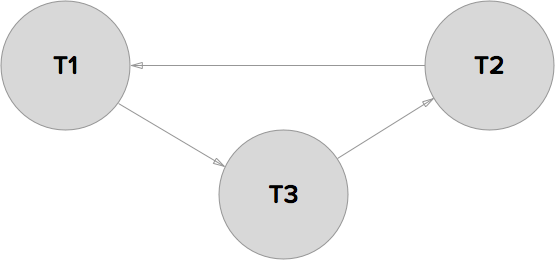
\includegraphics[width=0.7\textwidth]{schedule1.png}
    \caption{Precedence graph of schedule1 \label{precedencegraph1}}
\end{figure}

\begin{figure}[H]
    \centering
    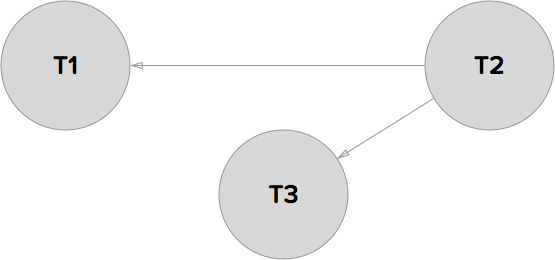
\includegraphics[width=0.7\textwidth]{schedule2.png}
    \caption{Precedence graph of schedule2 \label{precedencegraph2}}
\end{figure}

\subsection{Locking}

Schedule 1 could not have been generated by a scheduler using strict 2PL, since strict 2PL only allows conflict-serialisable schedules, and schedule 1 is not.
Schedule 2 could have been generated by a scheduler using strict 2PL. Figure \ref{schedule2strict2pl} shows the injected read/write lock operations that demonstrate this.

\begin{figure}
\begin{verbatim}
T1: S(X) R(X)                          X(Y) W(Y) C
T2:                         S(Z) R(Z)               X(X) W(X) X(Y) W(Y) C
T3:            X(Z) W(Z) C
\end{verbatim}
\caption{Injection of read/write lock operations into schedule 2\label{schedule2strict2pl}}
\end{figure}
